\documentclass[a4paper,UTF8]{article}
\usepackage{ctex}
\usepackage[margin=1.25in]{geometry}
\usepackage{color}
\usepackage{graphicx}
\usepackage{amssymb}
\usepackage{amsmath}
\usepackage{amsthm}
\usepackage{enumerate}
\usepackage{bm}
\usepackage{hyperref}
\usepackage{pgfplots}
\usepackage{epsfig}
\usepackage{color}
\usepackage{tcolorbox}
\usepackage{mdframed}
\usepackage{lipsum}
\usepackage{natbib}
\newmdtheoremenv{thm-box}{myThm}
\newmdtheoremenv{prop-box}{Proposition}
\newmdtheoremenv{def-box}{定义}
\newcommand{\derivative}[2]{\frac{\partial #1}{\partial #2}}
\newcommand{\suml}[2]{\sum\limits_{#1}^{#2}}

\setlength{\evensidemargin}{.25in}
\setlength{\textwidth}{6in}
\setlength{\topmargin}{-0.5in}
\setlength{\topmargin}{-0.5in}
% \setlength{\textheight}{9.5in}
%%%%%%%%%%%%%%%%%%此处用于设置页眉页脚%%%%%%%%%%%%%%%%%%    
\usepackage{fancyhdr}                                
\usepackage{lastpage}                                   
\usepackage{layout}                                     
\newtheorem*{solution}{Solution}

\footskip = 10pt 
\pagestyle{fancy}                    % 设置页眉                 
\lhead{2020年秋季}                    
\chead{高级机器学习}                                                
% \rhead{第\thepage/\pageref{LastPage}页} 
\rhead{作业三}                                                                                               
\cfoot{\thepage}                                                
\renewcommand{\headrulewidth}{1pt}  			%页眉线宽,设为0可以去页眉线
\setlength{\skip\footins}{0.5cm}    			%脚注与正文的距离           
\renewcommand{\footrulewidth}{0pt}  			%页脚线宽,设为0可以去页脚线

\makeatletter 									%设置双线页眉                                        
\def\headrule{{\if@fancyplain\let\headrulewidth\plainheadrulewidth\fi%
\hrule\@height 1.0pt \@width\headwidth\vskip1pt	%上面线为1pt粗  
\hrule\@height 0.5pt\@width\headwidth  			%下面0.5pt粗            
\vskip-2\headrulewidth\vskip-1pt}      			%两条线的距离1pt        
 \vspace{6mm}}     								%双线与下面正文之间的垂直间距              
\makeatother  

%%%%%%%%%%%%%%%%%%%%%%%%%%%%%%%%%%%%%%%%%%%%%%
\numberwithin{equation}{section}
%\usepackage[thmmarks, amsmath, thref]{ntheorem}
\newtheorem{myThm}{myThm}
\newtheorem*{myDef}{Definition}
\newtheorem*{mySol}{Solution}
\newtheorem*{myProof}{Proof}
\newtheorem*{myRemark}{备注}
\renewcommand{\tilde}{\widetilde}
\renewcommand{\hat}{\widehat}
\newcommand{\indep}{\rotatebox[origin=c]{90}{$\models$}}
\newcommand*\diff{\mathop{}\!\mathrm{d}}

\usepackage{multirow}

%--

%--
\begin{document}
\title{高级机器学习\\
大作业}
\author{丁豪\, 181220010} 
\maketitle
%%%%%%%% 注意: 使用XeLatex 编译可能会报错,请使用 pdfLaTex 编译 %%%%%%%

\section*{学术诚信}

本课程非常重视学术诚信规范,助教老师和助教同学将不遗余力地维护作业中的学术诚信规范的建立。希望所有选课学生能够对此予以重视。\footnote{参考尹一通老师\href{http://tcs.nju.edu.cn/wiki/}{高级算法课程}中对学术诚信的说明。}

\begin{tcolorbox}
	\begin{enumerate}
		\item[(1)] 允许同学之间的相互讨论,但是{\color{red}\textbf{署你名字的工作必须由你完成}},不允许直接照搬任何已有的材料,必须独立完成作业的书写过程;
		\item[(2)] 在完成作业过程中,对他人工作(出版物、互联网资料)中文本的直接照搬(包括原文的直接复制粘贴及语句的简单修改等)都将视为剽窃,剽窃者成绩将被取消。{\color{red}\textbf{对于完成作业中有关键作用的公开资料,应予以明显引用}};
		\item[(3)] 如果发现作业之间高度相似将被判定为互相抄袭行为,{\color{red}\textbf{抄袭和被抄袭双方的成绩都将被取消}}。因此请主动防止自己的作业被他人抄袭。
	\end{enumerate}
\end{tcolorbox}

\section*{作业提交注意事项}
\begin{tcolorbox}
	\begin{enumerate}
		\item[(1)] 请在LaTeX模板中{\color{red}\textbf{第一页填写个人的姓名、学号信息}};
		\item[(2)] 本次作业需提交该pdf文件、直接可以运行的源码,将以上几个文件压缩成zip文件后上传。zip文件格式为{\color{red}\textbf{学号.zip}},例如170000001.zip;pdf文件格式为{\color{red}\textbf{学号\_姓名.pdf}},例如170000001\_张三.pdf。
		\item[(3)] 未按照要求提交作业,或提交作业格式不正确,将会{\color{red}\textbf{被扣除部分作业分数}};
		\item[(4)] 本次作业提交截止时间为{\color{red}\textbf{1月8日23:59:59}}。除非有特殊情况(如因病缓交),否则截止时间后不接收作业,本次作业记零分。
	\end{enumerate}
\end{tcolorbox}

\newpage
\section{Introduction}
本次的作业为使用条件随机场(conditional random field,CRF)解决OCR(optical character recognition)问题。

在CRF模型中,有两种变量:我们要建模的隐藏变量和始终观察到的变量。对于OCR,我们要在观察的字符图像(也就是每个图像对应的像素数组)的情况下,对字符(例如“a”或“c”)进行建模。通常来说,未观察到的变量用$Y$表示,观察到的变量用$X$表示。CRF试图对$P(Y|X)$建模,即给定观察到的图像上字符的条件分布。该模型的结构如\ref{Fig.main1}下所示:
\begin{figure}[h] 
\centering
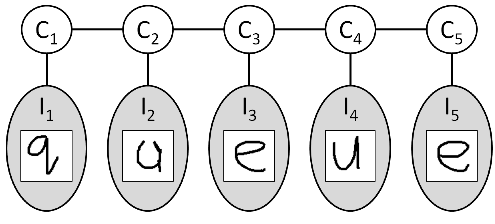
\includegraphics[width=0.7\textwidth]{figs/fig1.png} 
\caption{Markov Network} 
\label{Fig.main1}
\end{figure}

在CRF中,每个特征都对应一个权重$\theta_i$,在给定特征和权重的情况下,条件概率分布可以表示为:
\begin{equation}
P(\mathbf{Y} \mid \mathbf{x}: \theta)=\frac{1}{Z_{\mathbf{x}}(\theta)} \exp \left\{\sum_{i=1}^{k} \theta_{i} f_{i}\left(\mathbf{Y}, \mathbf{x}\right)\right\}\label{eq1}
\end{equation}

其中,$Z_x(\theta)$为配方函数
\begin{equation}
Z_{\mathbf{x}}(\theta) \equiv \sum_{\mathbf{Y}} \exp \left\{\sum_{i=1}^{k} \theta_{i} f_{i}\left(\mathbf{Y}, \mathbf{x}\right)\right\}
\end{equation}

在这次的任务中,一共有三类特征,三类特征均为指示函数,即满足条件时$f=1$,不满足时$f=0$:
\begin{itemize}
    \item $f_{i, c}^{C}\left(Y_{i}\right)$,指示是否$Y_i = c$
    \item $f_{i, j, c, d}^{I}\left(Y_{i}, x_{i j}\right)$,指示是否$Y_i=c,x_{ij}=d$
    \item $f_{i, c, d}^{P}\left(Y_{i}, Y_{i+1}\right)$,指示是否$Y_i=c,Y_{i+1}=d$
\end{itemize}

建立好模型,给定训练样本,我们就可以使用最大似然估计来进行学习:
\begin{equation}
    LL(\mathbf{x},\mathbf{Y},\theta) =\sum_{i=1}^{k} \theta_{i} f_{i}(\mathbf{Y}, \mathbf{x}) -\log \left(Z_{\mathbf{x}}(\theta)\right)\label{eq2}
\end{equation}

对于这个目标,我们可以使用梯度上升算法学习参数。

\section{Dataset}
本题中的数据集一共包含两个部分\texttt{trainset}和\texttt{testset}, 分别是训练集和测试集.训练集中有400个样本,测试集中有200个样本. 每个样本被存储在一个\texttt{txt}文件中, 第一行为对应的单词, 之后的每行为单词的每个字母对应的像素的状态.

\section{Assignment}
\begin{enumerate}
    \item 建立CRF模型,在训练集上进行训练,使用梯度上升的方法对模型参数进行求解,即求解公式\eqref{eq2}(注:不允许使用现有的CRF包,使用python实现)。
    \item 在模型训练完成后,在测试集上进行推断,评价模型的性能。
    \item 使用一些其他方法提高模型性能,可参考以下几个方面但不限于此:
    \begin{itemize}
        \item 提高模型表达能力:如在CRF图上添加新的连接。
        \item 缓解模型过拟合:如添加正则项。
        \item 加速模型训练过程:如权重共享。
    \end{itemize}
    \item 完成实验报告,主要包含具体的实现方法,如何复现运行代码,对模型的改进以及结果的分析等部分。
\end{enumerate}
\section {实验报告}
\subsection{记号与参考}
以下标记均针对“训练集”

$N$:总词数

$C$:所有可能出现的字母数量,通过程序统计可得其值为10,即len(alphabet)=10

$L_{i}$:$word_{i}$的长度,即$word_{i}$有$L_i$个字母

$F_i$:单词$word_i$的特征总量,即总共有$F_i$个0,1

$W^F$:观测状态矩阵,$W^F_{icd}$对应$f_{icd}(Y_i,Y_{i+1})$的系数

$W^T$:状态转移矩阵,$W^T_{ijcd}$对应$f_{ijcd}(Y_i,x_{ij})$的系数。特别地,在数据预处理阶段,在x矩阵前面添加一列全1,然后令$W^T_{i,0,c,1}$表示$f^C_{i,c}(Y_i)$对应的权重。这样我们就用$T$矩阵同时表示了两种特征值的权重。

以上$W^F,W^T$两者结合等同于本作业文档中的$\theta$,即模型参数。

\subsection{微分公式推导}
平均对数似然函数:
$$
\begin{aligned}
LL(x,Y,W^F,W^T)&=\frac 1 N \sum\limits_{i=1}^N \log P(y_i|x_i)\\
&=\frac{1}{N} \sum_{i=1}^{N}\left(\sum_{j=1}^{L_{i}} \sum_{f=1}^{F} W_{y_{j}^{(i)} f}^{F} x_{j f}^{(i)}+\sum_{j=1}^{L_{i}-1} W_{y_{j}^{(i)} y_{j+1}^{(i)}}^{T}-\log Z\left(W, x^{(i)}\right)\right)
\end{aligned}
$$

1)对数似然对观测状态矩阵$W_{cf}^{F}$的偏导数如下
$$
\begin{aligned}
\frac{\partial \mathcal{L}}{\partial W_{c^{\prime} f^{\prime}}}
&=\frac{\partial}{\partial W_{c^{\prime} f^{\prime}}} \frac{1}{N} \sum_{i=1}^{N}\left(\sum_{j=1}^{L_{i}} \sum_{f=1}^{F} W_{y_{j}^{(i)} f}^{F} x_{j f}^{(i)}+\sum_{j=1}^{L_{i}-1} W_{y_{j}^{(i)} y_{j+1}^{(i)}}^{T}-\log Z\left(W, x^{(i)}\right)\right)\\
&=\frac{1}{N} \sum_{i=1}^{N}\left(\sum_{j=1}^{L_{i}} \sum_{f=1}^{F} \mathbb{I}\left[y_{j}^{(i)}=c^{\prime}, f=f^{\prime}\right] x_{j f}^{(i)}-\sum_{\mathbf{y}} P(\mathbf{y} \mid \mathbf{x}) \mathbb{I}\left[y_{j}^{(i)}=c^{\prime}, f=f^{\prime}\right] x_{j f}^{(i)}\right) \\
&=\frac{1}{N} \sum_{i=1}^{N}\left( \sum_{j=1}^{k}\sum_{f=1}^{F}f_{j,f,c',f'}x_{jf} - \mathbb{E}_{P(y|x)} \left[ f_{j,f,c',f'}x_{jf} \right] \right)
\end{aligned}
$$


2)对数似然对状态转移矩阵$W_{cc}^{T}$的偏导数
\begin{equation*}
    \begin{aligned}
        \derivative{\mathcal{L}}{W_{cc'}} 
        &= \derivative{}{W_{cc'}} \frac{1}{N} \suml{i=1}{N} \left( \suml{j=1}{L_i} \suml{f=1}{F} W_{y_j^{(i)} f}^F x_{jf}^{(i)} + \suml{j=1}{L_i - 1} W_{y_j^{(i)} y_{j + 1}^{(i)}}^T - \log Z(W, x^{(i)}) \right) \\
        &= \frac{1}{N} \suml{i=1}{N} \left( \suml{j=1}{L_i - 1} \mathbb{I}[y_j^{(i)} = c, y_{j+1}^{(i)} = c'] - \suml{\mathbf{y}}{} P(\mathbf{y} | \mathbf{x}) \mathbb{I}[y_j^{(i)} = c, y_{j+1}^{(i)} = c'] \right) \\
        &= \frac{1}{N}  \sum_{i=1}^{N}\left(  \sum_{j=1}^{k}   f_{j,c,c'}^{P}(Y_{j}, Y_{j+1}) -   \mathbb{E}_{P(y | x)} \left[  f_{j, c,c'}^{P}(Y_{j}, Y_{j+1}) \right]    \right)
    \end{aligned}
\end{equation*}

\subsection{运行方式与代码实现}
本次实验参考了相关repo完成\footnote{https://github.com/deborausujono/crfocr}

运行方法:首先执行pip install -r requirements.txt安装依赖文件,然后运行181220010.py即可复现结果(分别对原始CRF以及加入了L2正则化后的CRF进行训练、测试、评估)

在项目中,crf.py文件实现了CRF模型的基本元素,包括势能函数、似然函数的计算、前文所述参数的梯度计算 以及根据生成好的CRF模型进行预测。crf\_with\_regular.py在以上基础上,增加了正则化损失,并将相应的梯度更新公式做了对应修改。util.py主要包含四个辅助函数,为数据读取、模型读取、模型存储以及计算测试集上的准确率。

CRF模型会首先计算每个节点势能函数并构建最大团的势能函数,然后使用前向后向算法进行信念传播来计算每一个节点的边缘概率分布,根据概率分布即可计算极大似然值。工程实现上,我们的目的是求解$W^F$与$W^T$两个矩阵,即状态权重和转移权重,通过极大似然估计后的梯度更新公式不断迭代更新,即可在有限步数内逐渐逼近其收敛值。在确定了损失函数及其导数之后,我们直接使用scipy.optimize.fmin\_l\_bfgs\_b函数进行优化,其可以在内存受限的情况下完成BFGS优化算法从而快速求解优化问题。
\end{document}